\begin{frame}
	\frametitle{Project Background}
		Nuclear fusion -- the energy of the future!
		\vfill
		\begin{columns}
			\column{0.43\textwidth}
			\centering{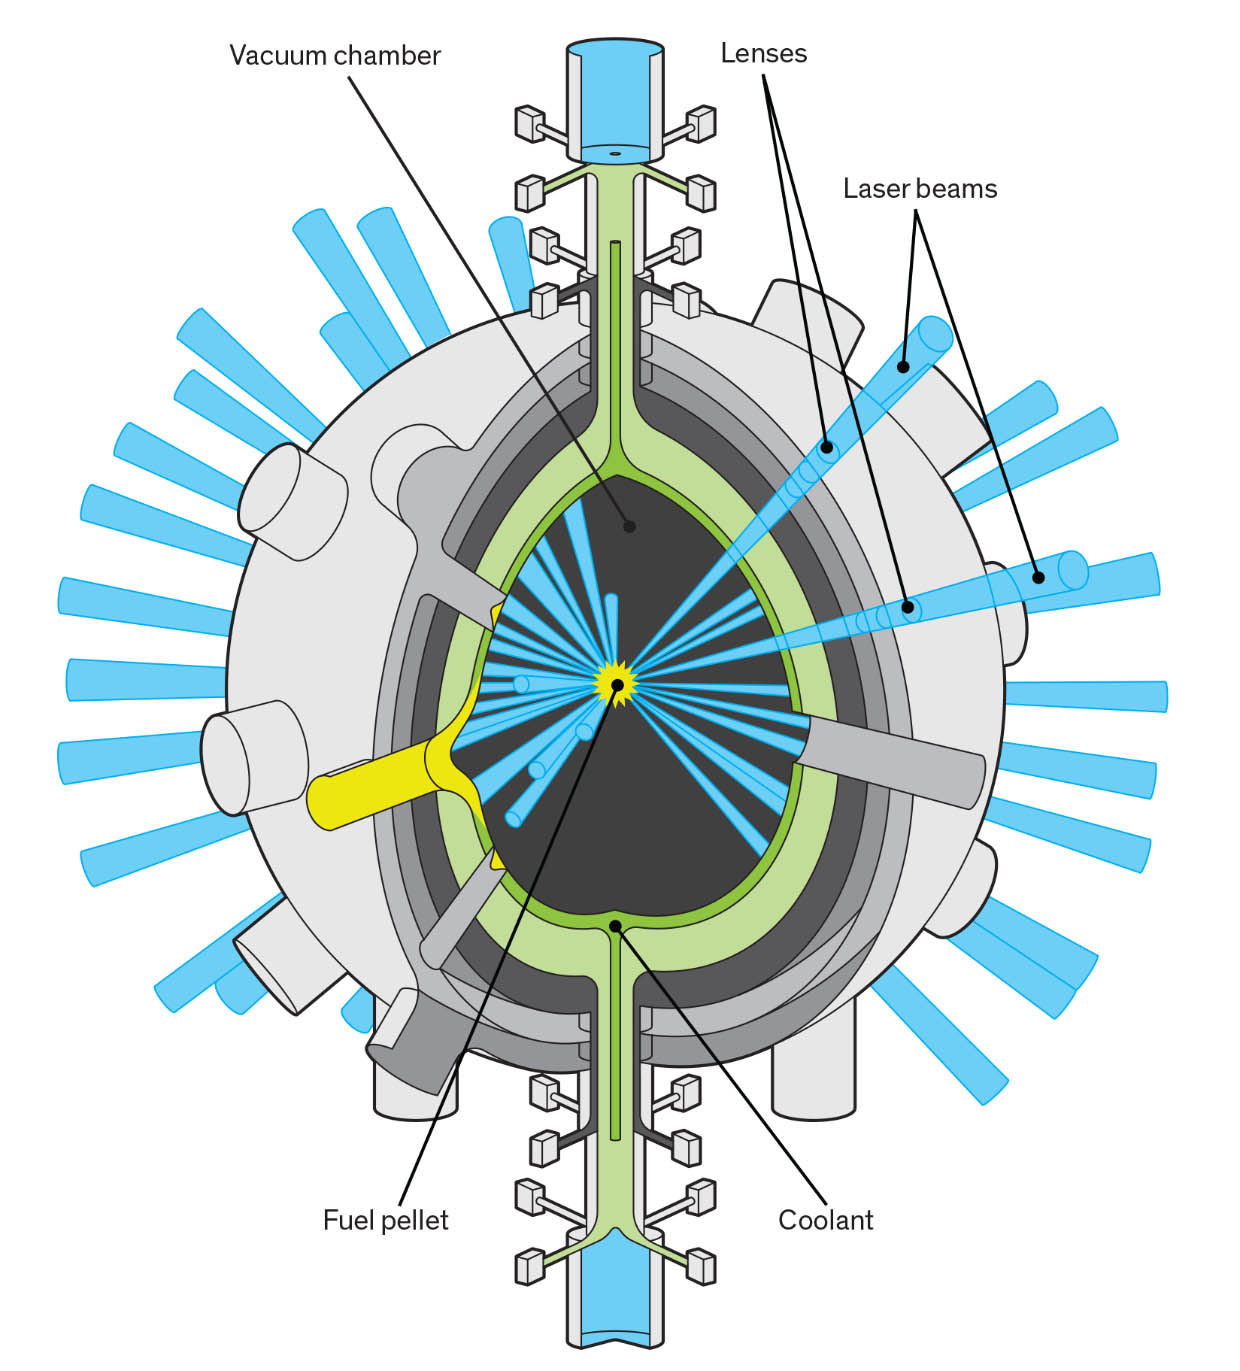
\includegraphics[width=\textwidth,trim={0 0 70pt 0},clip]{icf}}
			{\tiny
				Illustration by~Chris Philpot, courtesy of IEEE~Spectrum.
			}

			\column{0.57\textwidth}
			\begin{itemize}
				\setlength\itemsep{0.75em}
				\item Designing next-generation Inertial Confinement Fusion (ICF)
					facility.

				\item Search for optimal reactor design.

				\item \alert{Fueling} -- important for viability.

				\item Require fuel of 2~varieties:
				\begin{itemize}
					\setlength\itemsep{0.3em}
					\item Deuterium $^2$H -- abundant in~naturally-sourced water.
					\item Tritium $^3$H -- \alert{extremely rare.}
				\end{itemize}

				\item Modern reactors can generate tritium during operation.
			\end{itemize}
		\end{columns}
\end{frame}

\begin{frame}
	\frametitle{Problem Description}
	\alert{Tritium breeding blankets} convert neutron radiation to $^3$H fuel:
	\begin{align*}
		\isotope[1][0]{n} + \isotope[6][3]{Li} \rightarrow \isotope[3][1]{H} +
		\isotope[4][2]{He}
		\qquad\qquad
		\isotope[1][0]{n} + \isotope[7][3]{Li} \rightarrow \isotope[3][1]{H} +
		\isotope[4][2]{He} + \isotope[1][0]{n}
	\end{align*}
	\vfill
	$^3$H balance described by \alert{Tritium Breeding Ratio (TBR)} = $\cfrac{\text{fuel bred}}{\text{fuel consumed}}$
	\vspace{0.5em}
	\begin{itemize}
	    \item Depends on numerous geometric and material parameters.
	    \item Evaluated by \textit{Paramak} -- OpenMC neutronics simulation.
		\item Slow \ldots we want to consider as many reactor designs as possible!
	\end{itemize}
	\vfill
	\begin{block}{Our Challenge}
		\begin{center}
			Produce a \textit{fast} TBR surrogate that strongly approximates
			Paramak.
		\end{center}
	\end{block}
\end{frame}

\begin{frame}
	\frametitle{Data Generation}
	Produced datasets by sampling Paramak outputs over its
	7~discrete and 11~continuous input parameters at random.

	\begin{columns}[T]
		\column{0.35\textwidth}

		\vspace{10pt}

		Deployed at UCL's Hypatia cluster:
		\begin{itemize}
			\setlength\itemsep{0.5em}
			\item Created \alert{1M~points.}
			\item \alert{27 days} of runtime.
		\end{itemize}

		\vspace{13pt}

		2~classes of runs:
		\begin{itemize}
			\setlength\itemsep{0.5em}
			\item All parameters free.
			\item Discrete fixed, continuous free.
		\end{itemize}

		\vspace{10pt}


		\column{0.6\textwidth}
		\vspace{5pt}
		{\fontsize{8pt}{8pt}\selectfont
		\setlength\tabcolsep{3pt}
		\begin{tabular}{l|ll}
		\toprule
		{} & Parameter name & Domain\\
		\midrule
		\parbox[t]{2mm}{\hspace{-2pt}\multirow{12}{*}{\rotatebox[origin=c]{90}{Blanket}}}
		   & Breeder fraction\textsuperscript{\textdagger} & $[0,1]$\\
		   & Breeder \isotope[6]{Li} enrichment fraction & $[0,1]$\\
		   & Breeder material & $\{\text{Li}_2\text{TiO}_3, \text{Li}_4\text{SiO}_4\}$\\
		   & Breeder packing fraction & $[0,1]$\\
		   & Coolant fraction\textsuperscript{\textdagger} & $[0,1]$\\
		   & Coolant material & $\{\text{D}_2\text{O}, \text{H}_2\text{O}, \text{He}\}$\\
		   & Multiplier fraction\textsuperscript{\textdagger} & $[0,1]$\\
		   & Multiplier material & $\{\text{Be}, \text{Be}_{12}\text{Ti}\}$\\
		   & Multiplier packing fraction & $[0,1]$\\
		   & Structural fraction\textsuperscript{\textdagger} & $[0,1]$\\
		   & Structural material & $\{\text{SiC}, \text{eurofer}\}$\\
		   & Thickness & $[0,500]$\\
		\midrule
		\parbox[t]{2mm}{\hspace{-2pt}\multirow{6}{*}{\rotatebox[origin=c]{90}{First wall}}}
		   & Armour fraction\textsuperscript{\textdaggerdbl} & $[0,1]$\\
		   & Coolant fraction\textsuperscript{\textdaggerdbl} & $[0,1]$\\
		   & Coolant material & $\{\text{D}_2\text{O}, \text{H}_2\text{O}, \text{He}\}$\\
		   & Structural fraction\textsuperscript{\textdaggerdbl} & $[0,1]$\\
		   & Structural material & $\{\text{SiC}, \text{eurofer}\}$\\
		   & Thickness & $[0,20]$\\
		\bottomrule
		\end{tabular}
		}

		{\tiny
		Groups of parameters marked\textsuperscript{\textdagger\textdaggerdbl}
		are required to sum to 1.
		}

    \end{columns}
\end{frame}

\begin{frame}
	\frametitle{Methodology}
		Conventional regression task -- search for a cheap surrogate $\hat{f}(x)$ that
		\alert{minimizes dissimilarity} with an expensive function $f(x)$:

		\begin{itemize}
			\item
				Regression performance: mean absolute error, $\sigma$ of
				error, $R^2$, $R^2_\text{adj.}$
			\item
				Computational complexity:
				training \& prediction time / sample
		\end{itemize}

		\vspace{1em}
		2 approaches to solution:
		\vspace{-1em}

		\begin{columns}[t]
			\column{0.48\textwidth}
			\begin{block}{Decoupled Approach}
				\begin{enumerate}
					\item Collect training dataset.
					\item Use data to train a surrogate.
				\end{enumerate}
			\end{block}

			\hfill
			\column{0.48\textwidth}
			\begin{block}{Adaptive Approach}
				\begin{enumerate}
					\item Collect initial training dataset.
					\item Use data to train a surrogate.
					\item Collect more data in regions where surrogate performed poorly.
					\item Repeat steps 2 and 3.
				\end{enumerate}
			\end{block}
		\end{columns}


\end{frame}

